\section{Decision Trees}
\begin{frame}
   \frametitle{Decision Trees}
   Decision tree inducers provide an algorithm to solve classification and regression problems.
   \begin{itemize}
      \item  A binary decision tree $T$ splits the data: $s_T(x) = x_{i_T} \leq t_{T}$ unless $T$ is a leaf
      \item If $T$ is a leaf, it predicts $T(x) = c_T$ for some constant $c_T$
      \item If $T$ is not a leaf, it creates two subtrees $T_{left}$ and $T_{right}$, and predicts:
      \[   
      T(x) = 
            \begin{cases}

               T_{left}(x) &\quad\text{if}\:  s_T(x) = \text{TRUE} \\
               T_{right}(x) &\quad\text{if}\:  s_T(x) = \text{FALSE} \\
            \end{cases}
      \]
      \item This defines the capacity of the model
   \end{itemize}
\end{frame}


\begin{frame}
   \frametitle{Decision Trees - Example}
   \begin{center}
      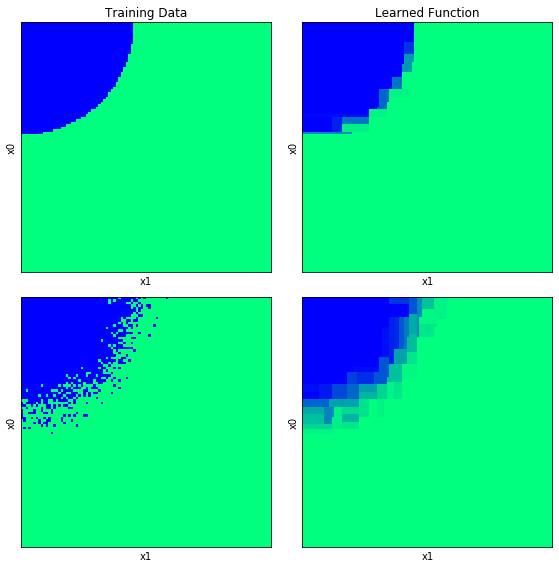
\includegraphics[height=150px]{img/true_vs_learned_regulartree.png}
   \end{center}
   \textit{Left:} Training data of an artificial classification problem. 
   \textit{Right:} Learned function of a decision tree
\end{frame}


\begin{frame}
   \frametitle{Decision Trees - Learning}  
   \begin{itemize}
   \item Fitting a tree is an optimization problem
   \item Many exact solutions are NP hard: e.g. finding a minimal tree that fits the data
   \item Instead of exact solutions: greedy algorithms (bottom up vs top down)
   \item Different loss functions have been proposed: \newline
   InformationGain, Gini Index,  Likelihood-Ratio Chi–Squared Statistics, DKM Criterion, Gain Ratio, ...- see \cite{rokach_decision_2005}
   \item This project evaluates the Information Bottleneck as loss function 
   \end{itemize}
\end{frame}



\begin{frame}[fragile]
   \frametitle{Decision Trees - Top Down}  
   \begin{lstlisting}[language=Python, basicstyle=\small]
class DecisionTree():
  def fit(self, X, Y):
    best_loss = infinity
    for d in range(X.shape[1]): # O(D) 
      loss, thresh, left_split, right_split = \
        best_split(X[:,d], Y) # O(N)
      if loss_d < best_loss:
        update best_loss, X_l, Y_l, X_r, Y_r, t_T, i_T
    if stopping_criterion is fulfilled:
      self.c_T = best_constant_estimator(Y)
      return self
    self.left = DecisionTree().fit(X_l, Y_l)
    self.right = DecisionTree().fit(X_r, Y_r)
    self.prune()
    return self
\end{lstlisting}

Time complexity: $O(N*D*depth(T)) \subseteq O(N*D*log_2(N))$
\end{frame}